\documentclass[../main.tex]{subfiles}
\graphicspath{{\subfix{../images/}}}

\begin{document}
\newcolumntype{C}{>{\centering\arraybackslash}p{0.3\textwidth}}

\subsection{Πεδία Ορισμού}

\renewcommand{\arraystretch}{1.5}
\tymin 0.3\textwidth
\begin{table}[H]
	\centering
	\begin{tabular}{C|C}
		\hline
		\textbf{Πεδίο ορισμού} & \textbf{Τύπος} \\
		\hline
		ταυτότητα              & INT(4)         \\
		ημερομηνία             & DATE()         \\
		όνομα                  & VARCHAR(25)    \\
		αλφαριθμητικό          & VARCHAR(25)    \\
		προσδιορισμός          & ENUM()         \\
		συντεταγμένες          & REAL()         \\
		\hline
	\end{tabular}
	\caption{Πεδία ορισμού της βάσης got-db}
\end{table}


\newenvironment{relation}[1]
{\renewcommand{\arraystretch}{1.4}
	\newcommand{\temp}{#1}
	\begin{table}[H]
		\centering
		\begin{tabular}[t]{*{2}{C}}
			\hline
			\multicolumn{2}{c}{Όνομα Σχέσης: \bf{#1}} \\
			\hline
			\multicolumn{2}{c}{\bf{Γνωρίσματα}}       \\
			\hline
			\textbf{Όνομα} & \textbf{Τύπος}           \\
			}
			{
			\hline
		\end{tabular}
		\caption{Σχέση \texttt{\temp}}
	\end{table}
}

\subsection{Σχέσεις}

\begin{relation}{character}
	character\_id         &  ταυτότητα\\
	name                  &  όνομα \\
	alias                 &  προσδιορισμός \\
	date\_of\_birth       &  ημερομηνία \\
	date\_of\_death       &  ημερομηνία \\
	titles                &  αλφαριθμητικό \\
\end{relation}

\begin{relation}{house}
	slogan                &  αλφαριθμητικό\\
	house\_name           &  όνομα \\
\end{relation}

\begin{relation}{non human}
	ID                &  ταυτότητα \\
	name              &  όνομα \\
	species           &  αλφαριθμητικό \\
\end{relation}

\begin{relation}{notable events}
	date              & ημερομηνία \\
	nickname          & όνομα \\
	Type\_of\_event   & προσδιορισμός \\
	outcome           & προσδιορισμός \\
\end{relation}

\begin{relation}{religion}
	name & όνομα \\
\end{relation}

\begin{relation}{location}
	x     & συντεταγμένες \\
	y     & συντεταγμένες \\
	name  & όνομα \\
\end{relation}

\subsection{Σχεσιακό Σχήμα}

\begin{figure}[H]
	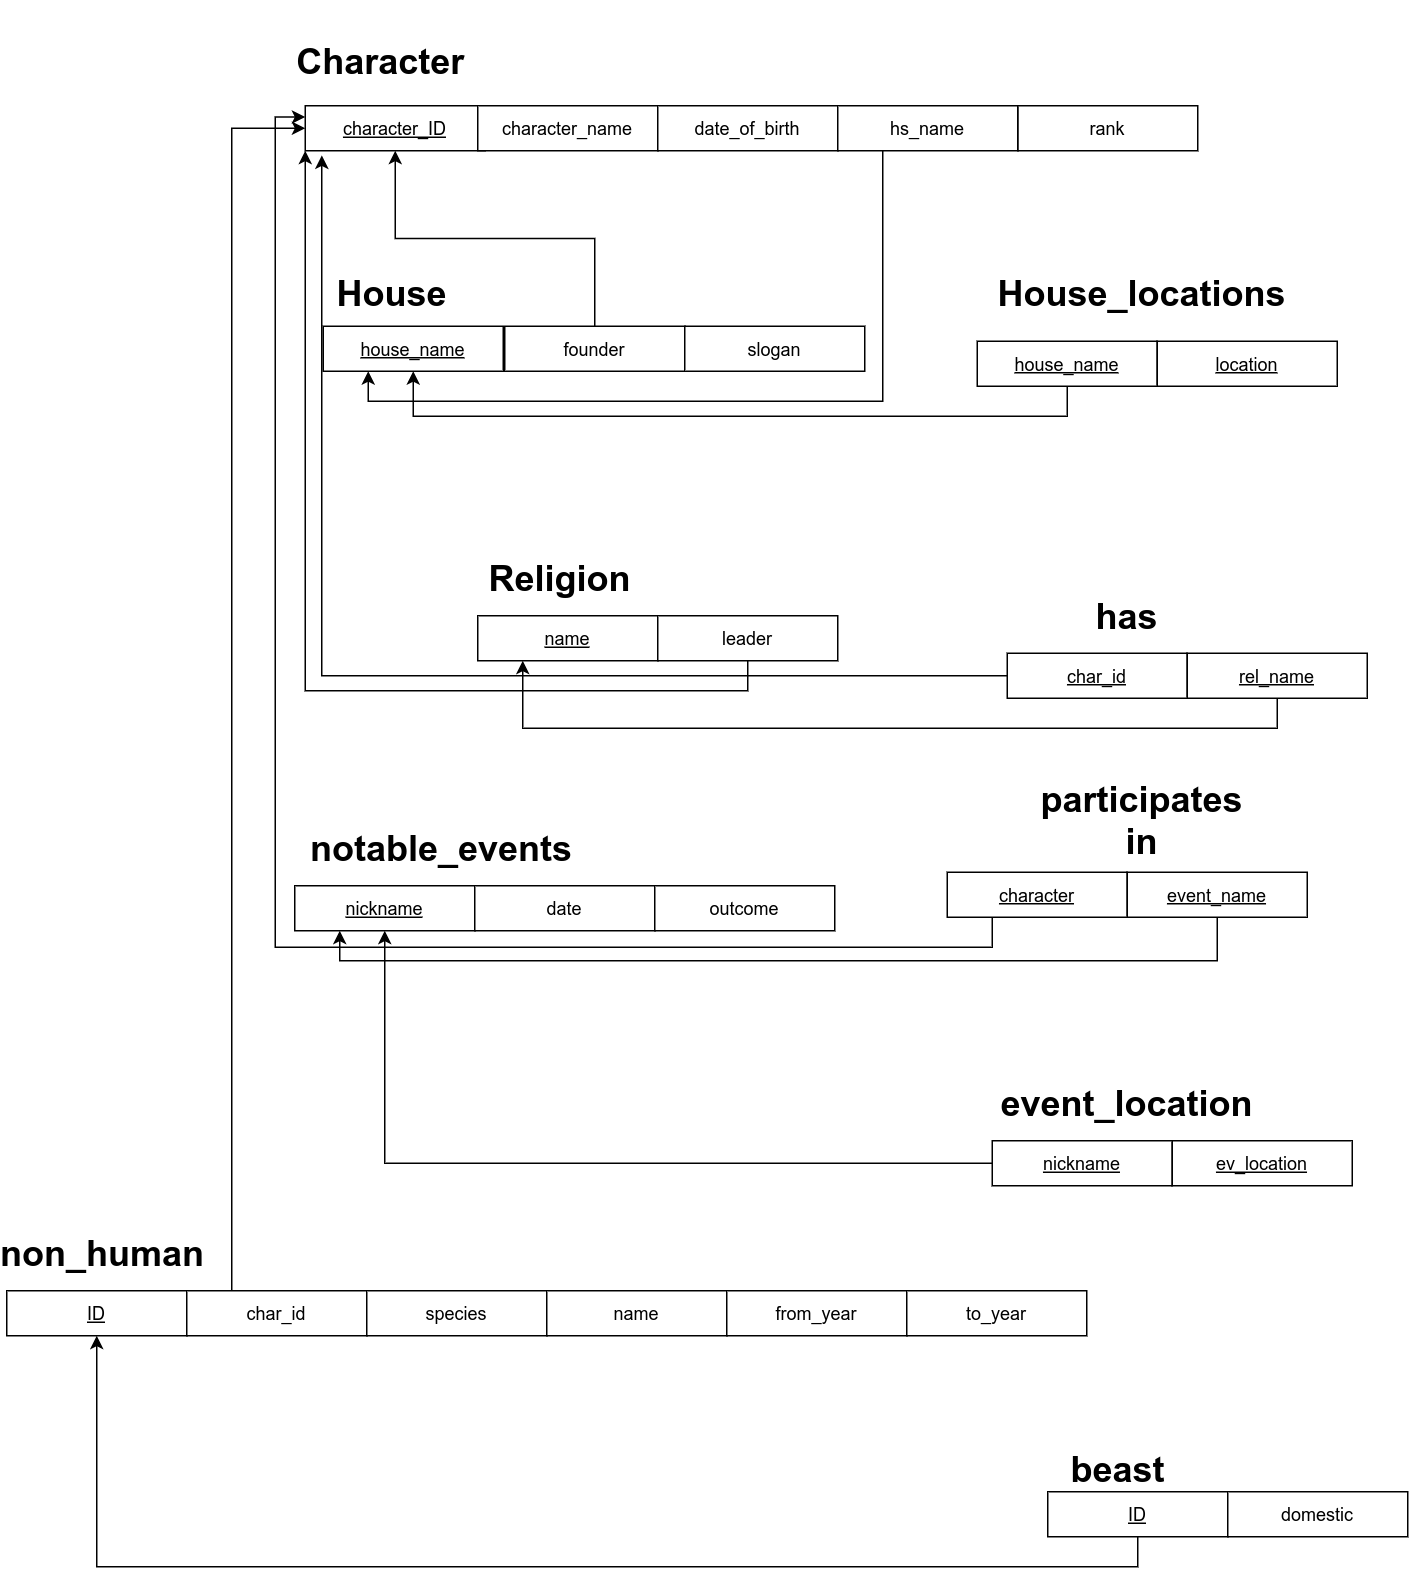
\includegraphics[width=\textwidth]{../images/relation_diagram.png}
	\caption{Σχεσιακό Σχήμα}
\end{figure}

\subsection{Όψεις}

% command for smaller subscripts
\newcommand{\tsub}[1]{\texttt{\tiny#1}}

Όψη που περιέχει όλους τους ηγέτες Θρησκειών.
\begin{equation}
	\bm{\rho}_{\tsub{LEADERS}}
	(
	\bm{\pi}_{\tsub{name,name}} (
	\bm{\pi}_{\tsub{leader\_id,name}}(\texttt{religion})
	\bowtie
	\bm{\pi}_{\tsub{id,name}}(\texttt{character})
	))
\end{equation}

\end{document}
